\chapter{Protocole expérimental}
	\section{Dispositif}
	\subsection{Hypothèses de travail}
	\label{ssec:hyp_travail}
	\par La première et principale hypothèse nécessaire au déroulement de cette expérimentation est que la luminance d'adaptation est considérée comme étant égale à la luminance de background: toutes les sources de luminosité parasites (voyants des ordinateurs, luminosité filtrant par la porte, ...) et la luminosité de la tache à visualiser sont jugées sans influences par rapport à la taille et à la puissance de la source lumineuse qu'est le background.
	
	\par Cette hypothèse est à un impact à plusieurs niveaux dans l'expérimentation: elle caractérise la valeur de la luminance sensée arriver à l'œil mais elle permet également une simplification dans l'équation de calcul des contrastes proposés aux sujets (voir plus bas, section \ref{ssec:contraste}).
	
	\par La seconde hypothèse est plus spécifique et concerne également l'équation de calcul du contraste. Rea et Ouellette utilisaient un filtre variable devant l'œil de leurs sujets pour atténuer l'intensité lumineuse et ont donc inclus une valeur de transmittance de ce filtre dans leur calcul du contraste. Nous n'utiliserons pas de filtre (l'expérimentation se déroule entièrement en 2D et donc sans lunettes stéréoscopique) et nous faisons l'hypothèse que cela revient à prendre une transmittance <<~parfaite~>>, c'est à dire de valeur maximale $T = 1$.
	
	\par Enfin, une dernière hypothèse concerne le mode opératoire directement. Même en ayant pris le plus grand soin possible avec un certain nombre de mesures préliminaires, on fait l'hypothèse qu'il est effectivement possible de reproduire l'expérimentation effectuée par Rea et Ouellette et de la <<~traduire~>> en Réalité Virtuelle.
	
	\par On rappelle que pour ce faire, on a calqué de la manière la fidèle possible notre mode opératoire sur le leur. Il existe néanmoins des différences, que ce soit sur l'outillage et la manière d'afficher les stimuli visuels mais également sur le nombre de sujets et surtout la quantité d'essai réalisés (dithyrambique du côté de Rea et Ouellette). L'influence du nombre d'essais réalisés est néanmoins nuancé par le fait qu'on effectue une vérification d'application du modèle contrairement à l'établissement d'une modèle à partir de zéro.
	
	\par Afin d'éviter tout biais de la part des projecteurs, le passage des sujets s'est fait dans une période de temps rapprochée et avec une période de chauffe de 1h avant le premier sujet de la journée pour que les projecteurs soient stabilisés, comme recommandé par la CIE (IEC 61966-6:2005).
	
	\subsection{Sujets \& matériel}
	\par On réunit un total de 32 sujets (Fig. \ref{fig:expe_sujets}) pour cette expérimentation, les même que pour l'étude expérimentale décrite dans la partie précédente (Cf.  \ref{chap:sdr_etude_experimentale}). Ces derniers sont volontairement choisis jeunes (entre 20 et 27 ans) pour minimiser l'impact de la dégradation de la vision avec l'âge. Tous les sujets ont donc une vision parfaite, ou corrigée et assimilée parfaite. La moyenne d'âge est de 25 ans, avec un écart-type de 1,8 ans.
	
	\par De même, les conditions matérielles sont identiques que pour la première expérimentation: dans un simulateur de type CAVE, les sujets sont assis dans un fauteuil de voiture, la tête bien calée dans l'appui-tête. Néanmoins, pour cette expérimentation, les sujets n'utilisent pas de lunettes stéréoscopiques. L'expérimentation se fait donc en affichage monoscopique. Les sujets sont placés de manière à avoir les yeux à 2 mètres du centre de l'écran <<~principal~>>, la face avant.
	
	\begin{figure}
		\centering
		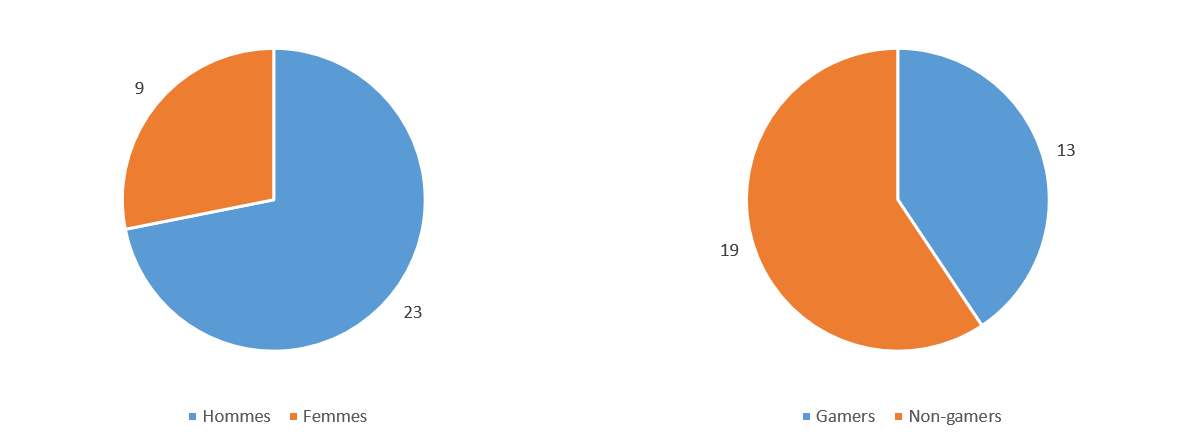
\includegraphics[scale=0.8]{Figures/SubjectsCharts}
		\caption{Répartitions des sujets pour les expérimentation de contraste/luminance et de comparaison objective/subjective.}
		\label{fig:expe_sujets}
	\end{figure}
	
	\subsection{Tâche à effectuer}
	\par L'expérimentation se déroulait en plusieurs étapes. La première consistait simplement en un petit questionnaire visant à relever quelques informations sur le sujet en lui même: âge, défauts éventuels et correction de vision, sexe, pratique des jeux vidéo. S'en suivait alors l'installation du sujet dans le simulateur et une explication de la tâche à effectuer pour l'expérimentation.
	
	\par De manière analogue aux expérimentations de Rea et Ouellette, les sujets devaient réagir à l'apparition de petits stimuli visuels sous la forme de disques uniformes de couleur sur un fond uniforme. La consigne était d'appuyer le plus vite possible, dès la perception du stimulus, sur un bouton spécifique (et toujours le même) d'une manette de console. Les couleurs uniformes des cibles et du fond étaient des nuances de gris choisies telles que les valeur de luminance aux niveaux des yeux et de contraste de l'un par rapport à l'autre soient parfaitement connues (voir plus bas).
	
	\par La seconde étape était une session blanche d'apparition de stimuli, c'est à dire sans stockage des mesures de temps de réaction, pour assurer une bonne prise en main de la tâche à effectuer, limiter le biais de la découverte et ainsi s'assurer que les temps de réactions mesurés sont les meilleurs. Le nombre de stimuli était légèrement plus faible que pour les sessions normales. La luminance choisie pour la session d'essai était différente de toutes les autres et choisie au milieu du spectre pour éviter tout biais d'habituation.
	
	\par Les étapes suivantes consistaient au déroulement des différentes sessions (voir le logigramme de déroulement global en Fig. \ref{fig:flowchart_expe_general}. Le sous-logigramme <<~CIBLES~>> est présenté en Fig. \ref{fig:flowchart_expe}), une pour chaque condition de luminance. Après chaque session, les conditions lumineuses étaient immédiatement réglées pour la session suivante puis un temps d'attente de 3 à 5 minutes était observé pour permettre aux yeux du sujet de s'adapter à la nouvelle luminance de fond. La consigne étaient de garder le regard sur les écrans du simulateur. Une fois le sujet adapté aux conditions lumineuses, il pouvait lancer de lui-même l'apparition des stimuli en appuyant sur un autre bouton spécifique de la manette de console.
	
	\begin{figure}
		\centering
		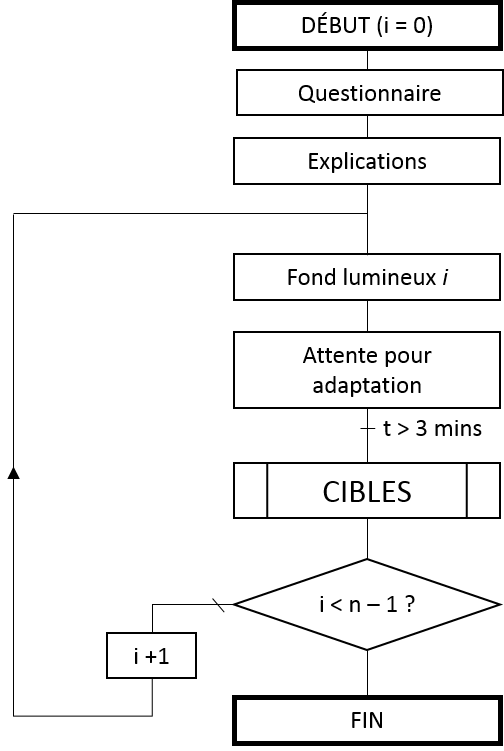
\includegraphics[scale=0.8]{Figures/FlowchartExpeRVPGeneral}
		\caption{Déroulement global de l'expérimentation contraste/lumimance.}
		\label{fig:flowchart_expe_general}
	\end{figure}
	
	\par L'ordre des luminances de fond proposées aux sujets était semi-aléatoire: distribution aléatoire pour chaque sujet mais de telle manière, qu'au global, autant de sujets aient rencontré la condition lumineuse \textit{p} en \textit{k-ième} position. Par exemple, autant de sujets ont eu la condition de luminance la plus sombre en première session, qu'en deuxième, qu'en troisième, etc.
	
	\par Tous les contrastes définis et possibles (voir plus bas, section \ref{ssec:contraste}) sont proposés au sujet pour chaque niveau de luminance. La présentation se fait dans un ordre aléatoire grâce à l'algorithme de mélange de Fisher-Yates (aussi appelé \textit{Algorithme P}, voir paragraphe suivant). Le mélange se fait à chaque nouvelle condition lumineuse mise en place: tous les sujets ont donc eu potentiellement une série différente à chaque fois et il n'était pas possible de prédire l'ordre avant de lancer l'apparition des cibles. L'apparition de chaque cible était espacée à chaque fois d'un temps incompressible de 1000~ms auquel s'ajoutait un temps aléatoire compris en 2000 et 4000~ms.
	
	\par Le principe de fonctionnement du mélange de Fisher-Yates, pour mélanger un tableau <<~T~>> de $n$ éléments (indices allant de $0$ à $n-1$), est le suivant:
	\begin{quote}
	 Pour i allant de n-1 à 1 faire :\\
       j $\leftarrow$ entier aléatoire entre 0 et i\\
       échanger T[j] et T[i]
	\end{quote}
	L'algorithme a une complexité linéaire et donne toutes les permutations avec la même probabilité. Il a été pensé de telle sorte que chaque élément du tableau ne bouge qu'une seule fois.
	
	\par Le déroulement d'une session, c'est à dire à un niveau de luminance donné, est résumé dans le logigramme en Fig. \ref{fig:flowchart_expe}.
	
	\begin{figure}
		\centering
		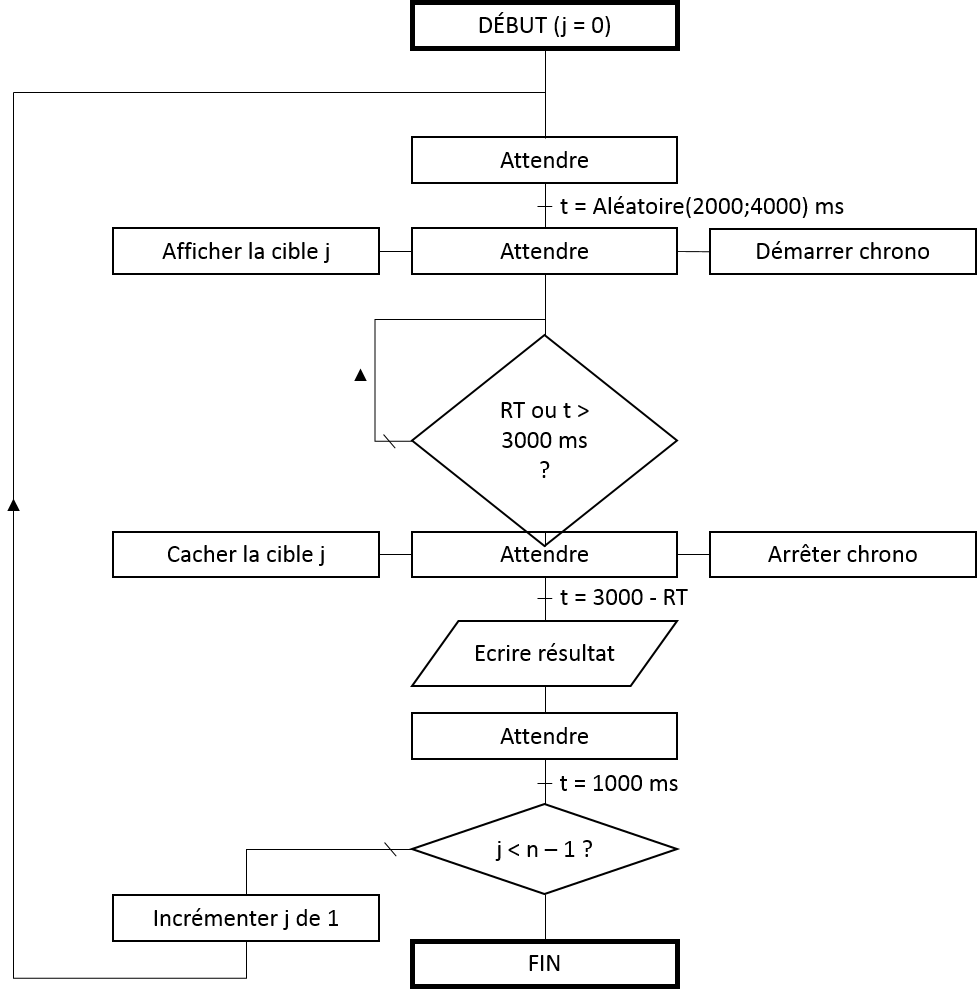
\includegraphics[scale=0.8]{Figures/FlowchartExpeRVP}
		\caption{Déroulement d'une session de mesure de temps de réactions pour une luminance de fond donnée.}
		\label{fig:flowchart_expe}
	\end{figure}
	
	\section{Choix des conditions expérimentales}
	\subsection{Luminance}
	\par Les conditions lumineuses de fond sont choisies de manière arbitraire, espacées régulièrement sur l'axe 0-255 bits (valeurs minimale et maximale pour coder une couleur sur 8 bits), d'une valeur d'au moins 32 bits (soit au moins 1/8ème de la plage totale de gris). On choisit évidemment les conditions extrêmes, à savoir la luminance liée à un background entièrement noir et la luminance liée à un background entièrement blanc. On choisit également la luminance associé au gris médian, c'est à dire 128 bits pour chacune des composantes R, G et B de la couleur affichée. Comme on a pu voir précédemment dans le chapitre sur les mesures préliminaires préalables au bon déroulement de l'expérimentation, les niveaux de luminance choisis sont associés aux niveaux de gris 0, 32, 80, 128, 176 et 255. On se limite à 6 conditions lumineuses différentes dans un soucis de temps requis pour faire passer les sujets sur tous les niveaux, pour tous les contrastes calculés.

	\par Tous nos niveaux de luminance sont compris dans les conditions pour lesquelles Rea et Ouellette ont établi leur modèle. Les limites de ce dernier sont fixées entre $0.53$ et $801~Td$~(Trolands\footnote{Le Troland est une unité de luminance pupillaire, définit par l'équation suivante: $Td = L \times p$ ; avec $L$ la luminance qui arrive à l'œil en $cd/m^2$ et $p$ la surface de la pupille en $mm^2$.}) vus à travers une pupille artificielle d'un diamètre de $2~mm$. Cela équivaut donc à des extrema lumineux à respectivement $0.17~cd/m^2$ et environ $255~cd/m^2$ ; tandis que nos extrema sont situés à $0.53~cd/m^2$ pour la condition la plus sombre et $42.82~cd/m^2$ pour la condition la plus claire.
	
	\subsection{Contraste}
	\label{ssec:contraste}
	\par Pour calculer les différents niveaux de contraste que l'on va proposer aux sujets, on se base sur la même équation de contraste utilisée par Rea et Ouellette (Eq. \ref{eq:rea_ouellette_contraste_2}). Cette dernière permet de calculer des valeurs de contraste comprises entre 0 et 1. On choisit, dans la mesure du possible (voir plus bas), de prendre des valeurs de contraste à intervalle régulier sur l'axe 0-1, espacés d'un dixième au maximum et d'un vingtième pour détailler la partie 0-0.25 de l'axe. Les valeurs de contraste cible/fond à atteindre sont donc: 0.05, 0.1, 0.15, 0.2, 0.25, 0.3, 0.4, 0.5, 0.6, 0.7, 0.8, 0.9 et 1 ; soit 13 valeurs. On peut atteindre ces valeurs de contraste par valeur <<~inférieure~>> c'est à dire avec une cible plus sombre que le fond (typiquement une cible grise sur fond blanc), mais également par valeur <<~supérieure~>>, c'est à dire avec une cible plus claire que le fond sur lequelle elle est affichée. Cela nous donne un total maximal théorique de 26 contrastes différents à tester par niveau de luminosité. Néanmoins, dans la plupart des cas, il n'est pas possible d'afficher tous les contrastes souhaités voire de ne pas pouvoir afficher du tout soit les contrastes <<~par valeur supérieure~>>, soit les contrastes <<~par valeur inférieure~>>. Typiquement, dans la condition de fond entièrement noir, il n'est pas possible d'afficher des cibles plus sombres et on ne peut donc avoir que des contrastes <<~supérieurs~>>.
	
	\begin{equation}
		C = \frac{\vert (T L_b + L_v) - (T L_t + L_v) \vert}{T L_b + L_v} = \frac{T \vert L_b - L_t \vert}{L_a}
		\label{eq:rea_ouellette_contraste_2}
	\end{equation}
	
	\par Il est maintenant nécessaire de déterminer quelle doit être la couleur du stimuli affiché, par rapport à la couleur du fond, pour atteindre précisément le contraste désiré. C'est ici que rentrent en jeux nos deux hypothèses préalablement établies (Cf. \ref{ssec:hyp_travail}): l'égalité entre la luminance d'adaptation et la luminance de background ($L_a = L_B$) d'un côté et la transmittance prise à sa valeur maximale ($T = 1$) de l'autre. On peut donc simplifier l'équation \ref{eq:rea_ouellette_contraste_2} et la transformer en une équation adaptée à notre dispositif (Eq. \ref{eq:contraste_p3i}), avec $L_b$ la luminance du fond et $L_t$ la luminance de la <<~target~>>, le stimuli:
	
	\begin{equation}
		C = \frac{T \vert L_b - L_t \vert}{L_a} \quad \Rightarrow \quad C = \frac{\vert L_b - L_t \vert}{L_b}
		\label{eq:contraste_p3i}
	\end{equation}
	
	\par Grâce aux régressions linéaires établies précédemment (cf. ), on peut écrire $L_b$ et $L_t$ comme des fonctions du niveau de gris dans notre simulateur, soit l'équation \ref{eq:luminance_egal_regression_background} avec $B$ la valeur entre 0 et 255 associée à la nuance de gris du fond. De même, l'équation \ref{eq:luminance_egal_regression_target} avec $T$ la valeur entre 0 et 255 associée à la nuance de gris de la cible, l'indice $B$ étant relatif à la nuance de gris du fond:
	
	\begin{equation}
		L_b = f\left( \frac{B}{255} \right)
		\label{eq:luminance_egal_regression_background}
	\end{equation}
	
	\begin{equation}
		L_t = f_B\left( \frac{T}{255} \right)
		\label{eq:luminance_egal_regression_target}
	\end{equation}
	
	\par On obtient donc, au final, l'équation suivante qui nous permet de calculer avec précision la valeur de la nuance de gris de la cible à afficher lorsque qu'on connaît la nuance de gris du fond pour afficher un contraste choisi (Eq. \ref{eq:contraste_p3i_regression}):
	
	\begin{equation}
		C = \frac{\vert f\left( \frac{B}{255} \right) - f_B\left( \frac{T}{255} \right) \vert}{f\left( \frac{B}{255} \right)}
		\label{eq:contraste_p3i_regression}
	\end{equation}
	
	\par Néanmoins, comme décrit précédemment, on souhaite pouvoir calculer des contrastes <<~supérieurs~>> et <<~inférieures~>>, hors cette équation ne fonctionne que si la luminance de fond est supérieure à la luminance de la cible. Il faut donc adapter l'équation pour calculer les contrastes <<~supérieurs~>> (Eq. \ref{eq:contraste_p3i_regression_alt}):
	
	\begin{equation}
		C = \frac{\vert f\left( \frac{B}{255} \right) - f_B\left( \frac{T}{255} \right) \vert}{f_B\left( \frac{T}{255} \right)}
		\label{eq:contraste_p3i_regression_alt}
	\end{equation}
	
	\par On présente dans les tables suivantes les valeurs de nuances de gris nécessaires pour afficher les contrastes par valeur <<~supérieure~>> (Tab. \ref{tab:contraste_sup}) et par valeur <<~inférieure~>> (Tab. \ref{tab:contraste_inf}). La première ligne donne les contrastes obtenus, la première colonne les niveaux de gris en background et le reste du tableau le niveau de gris du stimuli. On peut voir que notamment dans le cas du background le plus sombre, les valeurs ne varient que de 1 bit et donc qu'il ne serait pas possible avec notre système d'avoir un pas de variation du contraste plus fin. On remarque que, pour les contrastes supérieurs 0.15 et 0.2 sur fond noir, la même valeur de gris est associée. Ce cas est unique et vient du fait que la régression linéaire est continue alors que l'on cherche des valeurs ponctuelles, pour des valeurs très proches ni l'arrondi ni la troncature ne permettent de les départager. On a donc ignoré une des deux valeurs pendant l'expérimentation.
	
	\begin{table}[h]	
		\centering
		\caption{Valeurs des nuances de gris du stimulus nécessaire pour afficher un contraste par valeur supérieur désiré.}
		\label{tab:contraste_sup}
		\begin{tabular}{c|ccccccccccccc}
			\textbf{C} & \textbf{0.05} & \textbf{0.1} & \textbf{0.15} & \textbf{0.2} & \textbf{0.25} & \textbf{0.3} & \textbf{0.4} & \textbf{0.5} & \textbf{0.6} & \textbf{0.7} & \textbf{0.8} & \textbf{0.9} & \textbf{1}\\
			\hline
			\textbf{0} & 16  & 17  &  18  & 18 & 19 & 20 & 21 & 22 & 23 & 24 & 25 & 26 & 27\\
			\textbf{32} & 33 & 35 & 36 & 37 & 38 & 39 & 41 & 42 & 44 & 46 & 47 & 49 & 50\\
			\textbf{80} & 85 & 88 & 90 & 93 & 95 & 98 & 102 & 106 & 110 & 114 & 118 & 121 & 125\\
			\textbf{128} & 133 & 138 & 142 & 147 & 151 & 156 & 164 & 172 & 180 & 187 & 195 & 203 & 211\\
			\textbf{176} & 182 & 190 & 198 & 206 & 214 & 222 & 239\\
			\textbf{255}\\
		\end{tabular}
	\end{table}
	
	\begin{table}[h]	
		\centering
		\caption{Valeurs des nuances de gris du stimulus nécessaire pour afficher un contraste par valeur supérieur désiré.}
		\label{tab:contraste_inf}
		\begin{tabular}{c|ccccccccccccc}
			\textbf{C} & \textbf{0.05} & \textbf{0.1} & \textbf{0.15} & \textbf{0.2} & \textbf{0.25} & \textbf{0.3} & \textbf{0.4} & \textbf{0.5} & \textbf{0.6} & \textbf{0.7} & \textbf{0.8} & \textbf{0.9} & \textbf{1}\\
			\hline
			\textbf{0}\\
			\textbf{32} & 31 & 29 & 28 & 27 & 26 & 24 & 22 & 19 & 15\\
			\textbf{80} & 79 & 76 & 74 & 71 & 69 & 66 & 61 & 57 & 52 & 47 & 52 & 37 & 31\\
			\textbf{128} & 123 & 118 & 114 & 109 & 105 & 101 & 93 & 85 & 78 & 70 & 62 & 52 & 40\\
			\textbf{176} & 167 & 160 & 153 & 147 & 140 & 135 & 123 & 112 & 101 & 91 & 79 & 67 & 50\\
			\textbf{255} & 232 & 218 & 206 & 196 & 186 & 177 & 161 & 146 & 132 & 117 & 102 & 86 & 66\\
		\end{tabular}
	\end{table}
	
	\par A titre d'exemple, lorsque la couleur de background est un gris 128 (Code RGB = (128, 128, 128), pour afficher un stimulus contrasté par valeur supérieure à 0.3, il faut que la cible soit un gris 156, c'est à dire avec un code RGB égal à (156, 156, 156). 
	
	\par Maintenant que l'on a choisi les luminances de fond, que l'on sait à quelle nuance de gris elles correspondent, qu'on a choisi les contrastes que l'on voulait afficher et que l'on sait à quelles couleurs ils correspondent, on peut passer à la partie purement expérimentale et inviter des sujets à confronter leurs temps de réaction à l'apparition de nos stimuli calibrés. Les résultats théoriques et pratiques de ces expérimentations sont présentés dans le chapitre suivant.
	
\chapter{Résultats}
	\section{Prédictions du modèle théorique}
	\par On calcule les temps de réactions prévus par le modèle que l'on chercher à vérifier. Ces temps sont en millisecondes (ms). On présente ces résultats sous forme de tableau avec en colonne les différents contrastes affichés et en ligne les niveaux de gris du background (Table \ref{tab:theoretical_reaction_times}).
	
	\par On laisse une case vide dans le tableau lorsque le modèle n'est pas capable de prédire un temps de réaction: le sujet n'est pas sensé réussir à distinguer le stimuli par rapport au fond. On remarque également que certaines valeurs sont complètement démesurées (typiquement, il faudrait théoriquement 25 secondes à un individu pour distinguer un stimuli contrasté à 0.20 sur un fond gris 80). Ces valeurs sont dues à un diviseur très proche de zéro dans les formules utilisée qui rend les valeurs de contraste proches du contraste seuil théorique très volatiles.
	
	\par Pour l'ensemble des conditions, les valeurs de temps de réaction (une fois passé le seuil limite de contraste) croissent régulièrement jusqu'à tendre vers une asymptote pour les conditions les plus lumineuses.
	
	\begin{table}[h]	
		\centering
		\caption{Temps de réaction théoriques (en ms) prédits par le modèle de Rea et Ouellette.}
		\label{tab:theoretical_reaction_times}
		\begin{tabular}{c|cccccc}
			\textbf{C/L} & \textbf{0} & \textbf{32} & \textbf{80} & \textbf{128} & \textbf{176} & \textbf{255}\\
			\hline
			\textbf{0.05}\\
			\textbf{0.10}\\
			\textbf{0.15} &  &  &  &  & $10865$ & $3594$\\
			\textbf{0.20} &  &  & $25435$ & $1924$ & $1429$ & $1212$\\
			\textbf{0.25} &  &  & $1686$ & $1041$ & $912$ & $839$\\
			\textbf{0.30} &  &  & $1039$ & $788$ & $725$ & $685$\\
			\textbf{0.40} &  & $2663$ & $696$ & $596$ & $568$ & $549$\\
			\textbf{0.50} &  & $1272$ & $577$ & $517$ & $499$ & $546$\\
			\textbf{0.60} &  & $929$ & $517$ & $473$ & $549$ & $449$\\
			\textbf{0.70} &  & $773$ & $481$ & $446$ & $434$ & $425$\\
			\textbf{0.80} & $4451$ & $684$ & $456$ & $426$ & $416$ & $409$\\
			\textbf{0.90} & $2448$ & $626$ & $439$ & $412$ & $403$ & $396$\\
			\textbf{1.00} & $1720$ & $585$ & $425$ & $402$ & $393$ & $387$\\
		\end{tabular}
	\end{table}
	
	\section{Mesures réelles}
	\par Les mesures réelles sont mesurées directement par le logiciel qui affiche les stimuli. Les résultats sont ensuite écrits dans un fichier externe que l'on récupère et que l'on traite ensuite dans Excel. La précision des mesures est limitée par le nombre d'images par seconde auquel le programme tourne: à chaque image, le programme vérifie si le sujet appuie ou non sur le bouton de détection et stoppe le chronomètre le cas idoine. Toute action entre 2 images est donc ignorée jusqu'au calcul suivant. C'est pourquoi la précision des mesures de temps est précise à un demi-temps inter-image près. Le programme fonctionnant à 120 images par secondes (la limite se faisant au niveau du projecteur), la précision est donc de 1/240ème de seconde soit $4~ms$. Au regard des valeurs attendues (les temps les plus rapides prévus dans nos conditions par le modèle sont de $400~ms$) cela représente une erreur de 1\% qui peut donc être négligée.
	
	\begin{table}[h]	
		\centering
		\caption{Temps de réaction moyens réels (en ms) mesurés pendant l'expérimentation et leurs écart-types moyens.}
		\label{tab:real_reaction_times}
		\begin{tabular}{c|cccccc}
			\textbf{C/L} & \textbf{0} & \textbf{32} & \textbf{80} & \textbf{128} & \textbf{176} & \textbf{255}\\
			\hline
			\textbf{0.05} & $465 \pm 58$ & $2013 \pm 429$ & $670 \pm 112$ & $572 \pm 314$ & $500 \pm 290$ & $450 \pm 155$\\
			\textbf{0.10} & $474 \pm 98$ & $663 \pm 447$ & $450 \pm 86$ & $421 \pm 66$ & $434 \pm 71$ & $406 \pm 50$\\
			\textbf{0.15} & $474 \pm 85$ & $553 \pm 286$ & $439 \pm 78$ & $421 \pm 85$ & $434 \pm 99$ & $404 \pm 48$\\
			\textbf{0.20} & $468 \pm 67$ & $531 \pm 323$ & $418 \pm 48$ & $422 \pm 87$ & $407 \pm 75$ & $432 \pm 88$\\
			\textbf{0.25} & $465 \pm 158$ & $479 \pm 63$ & $415 \pm 68$ & $101 \pm 50$ & $141 \pm 62$ & $398 \pm 92$\\
			\textbf{0.30} & $475 \pm 141$ & $507 \pm 215$ & $423 \pm 73$ & $399 \pm 53$ & $412 \pm 63$ & $393 \pm 72$\\
			\textbf{0.40} & $443 \pm 74$ & $457 \pm 59$ & $451 \pm 221$ & $400 \pm 59$ & $406 \pm 63$ & $396 \pm 52$\\
			\textbf{0.50} & $440 \pm 44$ & $461 \pm 78$ & $418 \pm 71$ & $409 \pm 62$ & $394 \pm 42$ & $415 \pm 67$\\
			\textbf{0.60} & $440 \pm 58$ & $451 \pm 66$ & $405 \pm 52$ & $396 \pm 52$ & $403 \pm 6$ & $402 \pm 81$\\
			\textbf{0.70} & $466 \pm 94$ & $450 \pm 80$ & $416 \pm 72$ & $394 \pm 49$ & $408 \pm 57$ & $390 \pm 48$\\
			\textbf{0.80} & $432 \pm 68$ & $443 \pm 67$ & $402 \pm 46$ & $405 \pm 80$ & $394 \pm 48$ & $398 \pm 67$\\
			\textbf{0.90} & $464 \pm 79$ & $440 \pm 61$ & $404 \pm 58$ & $402 \pm 61$ & $400 \pm 64$ & $399 \pm 77$\\
			\textbf{1.00} & $448 \pm 152$ & $426 \pm 41$ & $403 \pm 52$ & $401 \pm 77$ & $398 \pm 64$ & $371 \pm 48$\\
		\end{tabular}
	\end{table}
	
	\par Les moyennes des temps de réaction mesurés et leurs écart-types sont listés dans la Table \ref{tab:real_reaction_times}. Etant donné que la population de sujet était supérieure ou égale à 30, on a pu calculer l'écart type réel (Pearson) et non pas un estimateur. Les valeurs si situent entre $371~ms$ et $670~ms$ avec une moyenne des moyennes (en excluant les valeurs divergentes, voir plus loin) à $437~ms$ (écart-type = $53~ms$) et un écart-type moyen de $96~ms$ (écart-type = $82~ms$). On nota particulièrement la valeur de temps de réaction ($2013~ms$) atteinte pour un contraste de $0.05$ et une luminance de fond de $0.41~cd/m^2$).
	
	\par La performance R est définie telle que l'inverse du temps de réaction RT: $R = 1/RT$. On l'utilise, plutôt que le temps de réaction, pour décrire les résultats obtenus: la performance augmente quand le temps de réaction diminue et inversement, ce qui semble plus logique. Les figures \ref{fig:results_rvp_1}, \ref{fig:results_rvp_2} et \ref{fig:results_rvp_3} montrent, pour chaque condition lumineuse, la comparaison entre la performance théorique que l'on devrait avoir et la performance réelle mesurée pendant l'expérimentation. Les points correspondant à une performance nulle décrivent les points en dessous du seuil de perception: le temps de réaction est alors <<~infini~>> et donc son inverse (la performance) tend vers 0.
	
	\begin{figure}
		\centering
		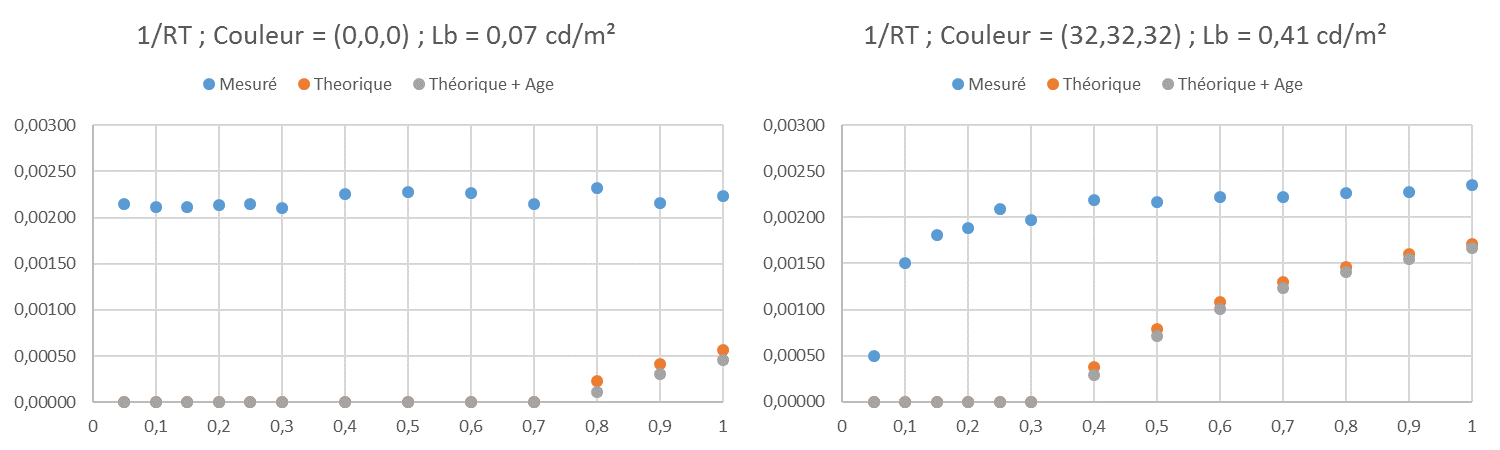
\includegraphics[width=\linewidth]{Figures/ResultsRVP_1}
		\caption{Performance théorique et réelle pour l'expérimentation de détection des stimuli contrastés, conditions 0 et 32.}
		\label{fig:results_rvp_1}
	\end{figure}
	
	\begin{figure}
		\centering
		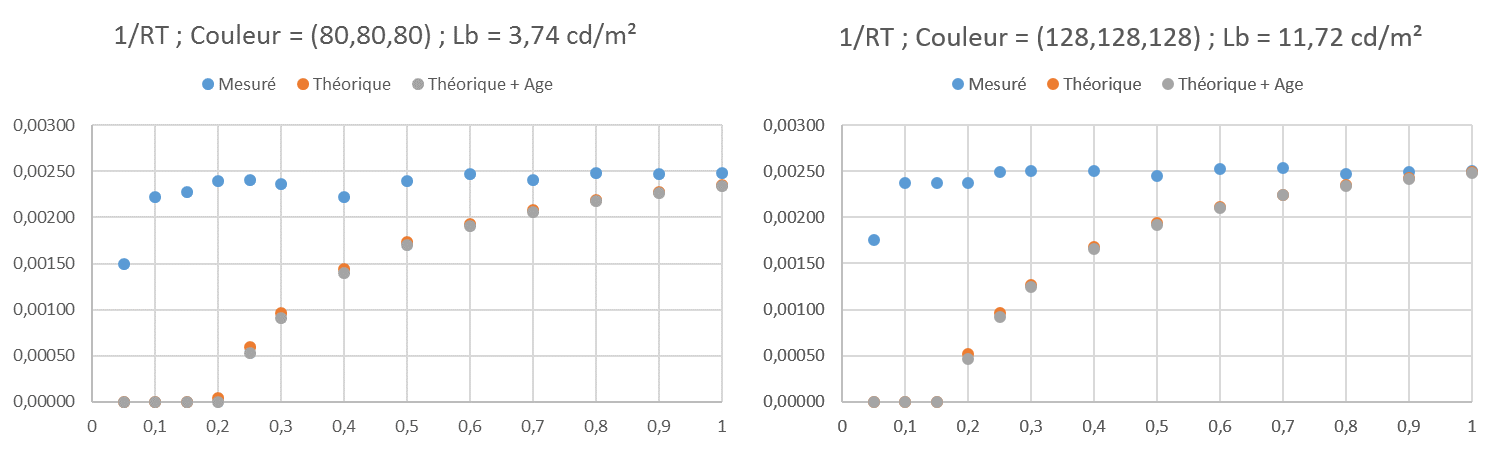
\includegraphics[width=\linewidth]{Figures/ResultsRVP_2}
		\caption{Performance théorique et réelle pour l'expérimentation de détection des stimuli contrastés, conditions 80 et 128.}
		\label{fig:results_rvp_2}
	\end{figure}
	
	\begin{figure}
		\centering
		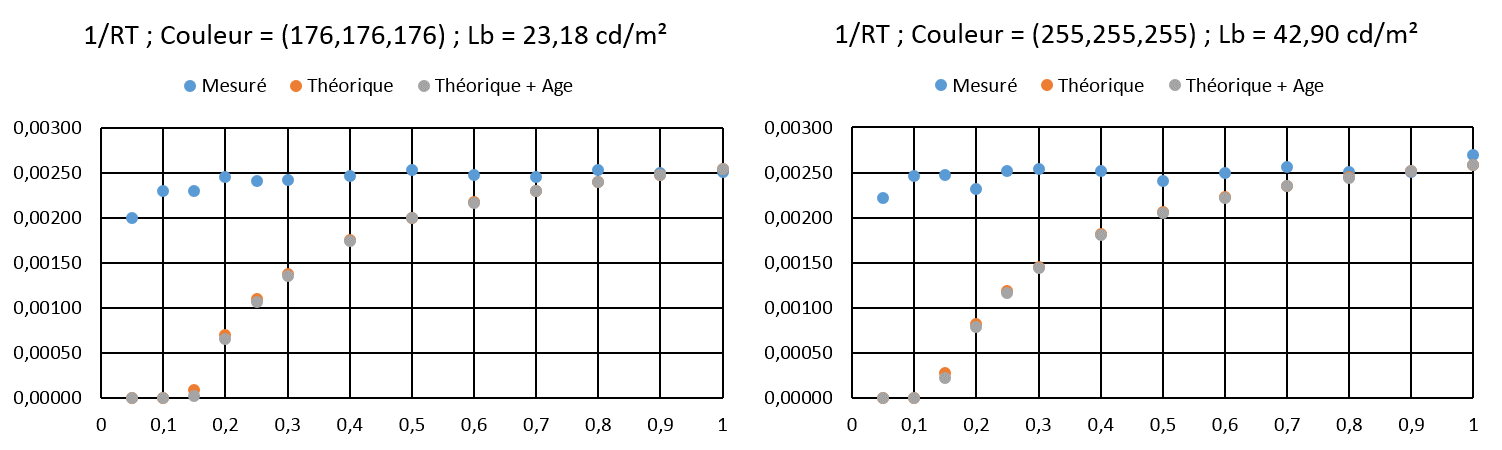
\includegraphics[width=\linewidth]{Figures/ResultsRVP_3}
		\caption{Performance théorique et réelle pour l'expérimentation de détection des stimuli contrastés, conditions 176 et 255.}
		\label{fig:results_rvp_3}
	\end{figure}
		
	\section{Analyse et discussion}
	\par Le premier résultats qui frappe est qu'alors que le modèle de Rea prévoit que certains stimulis ne doivent pas être vus (étant en dessous du seuil), nos sujets ont été capables de voir toutes les taches lumineuses qui leur étaient présentées, et ce, quelles que soient les conditions de luminance et de contraste.
	
	\par Deuxièmement, la différence entre le comportement théorique prévu et les mesures sur nos sujets est radicale. Alors que la performance est sensée augmenter avec le contraste et la luminance, il apparait que notre performance est toujours constante. Les sujets avaient un temps de réaction globalement identique avec des conditions lumineuses pourtant très différentes. En se fiant aux prédictions du modèle de Rea et Ouellette, les sujets ne devraient pas être aussi capables: il devraient d'abord ne rien voir puis, alors que la luminance et surtout le contraste augmentent, être de plus en plus bons. Les comportements étant aussi radicalement opposés, nous n'avons pas jugé nécessaire de déployer une méthode statistique pour vérifier si les échantillons de mesure (mesures théoriques et mesures pratiques) étaient appariés.
	
	\par Au final, nos résultats ne correspondent pas du tout avec les prévisions de Rea et Ouellette mais convergent néanmoins vers les même valeurs. Bien que nous ayons fait de notre mieux pour traduire l'expérimentation initiale dans notre simulateur, il existe néanmoins toujours des différences fondamentales entre les prévisions et les mesures.
	
	\par La différence principale entre les deux dispositifs expérimentaux et la quantité de lumière qui arrive à l'œil, et la quantité de sources lumineuses. Du côté de Rea et Ouellette, la seule source de lumière était un petit écran situé à une distance de $1.68~m$ du sujet, en plus d'une lumière dirigée directement dans l'œil au moyen d'un miroir semi transparent. De plus, la quantité de lumière arrivant à l'œil était également contrôlée avec un filtre devant l'œil. De notre côté, la lumière est issue d'écrans géants entourant le sujet ainsi qu'une multitude de petites lumières indirectes: les projecteurs émettent leur lumière en direction des écrans. Nous n'avons pas braqué de lumière directement dans l'œil de nos sujets et nous n'avons pas utilisé de filtre pour atténuer la lumière (tout en plaçant néanmoins des hypothèses). Enfin, Rea et Ouellette filtraient la lumière arrivant à l'œil au moyen d'un filtre mais le montage ne semble pas être complètement étanche et a pu laisser passer de la lumière parasite non atténuée.
	
	\par Ainsi, de part la comparaison entre nos résultats et les prédiction, à notre avis, le modèle de Rea et Ouellette ne devrait pas être utilisé dans le domaine de la Réalité Virtuelle pour déterminer la performance de l'œil (par rapport à la modélisation de la vision humaine), avec pour seule base le contraste et la luminance.
